\section{Database caching}

WordPress-powered sites are doing quite a lot of queries into the database on each load. If an user installs plugins and uses a more complex theme, querying the database starts to become a bottleneck. It can take up to 200-300 milliseconds from each page load. When there is a high traffic coming to a site, database stops being able to process all the queries and PHP processing halts (queries are synchronized).

A solution to this problem is to store (cache) the results of the database queries so when the same query is run again, the stored data, instead of querying the database, is returned.

WordPress comes with a object cache API in its Core. All Core functions and methods querying the database (such as get\_option, get\_posts, etc) use this object cache API. However, as WordPress supports wide range of hosts and server versions, this API caches the data only during the request procesing. That means that when the data are queried for the first time, they get stored in a PHP array. Next time they are retrieved (during the same request processing) from that array.

Fortunately, native WordPress object caching API can be swapped for more robust caching mechanisms. It is done by writing an object-cache.php file, putting it into the wp-content directory. If WordPress detects this file, it will use the functions defined from it instead of loading its own object cache API code.

There are two main caching mechanisms: WordPress Transient API and in-memory caching.

WordPress Transient API works by storing the cached data back into the database as a serialized PHP array. Instead of having to perform a complex database query, the data is simply retrieved from the database and unserialized back into a PHP array. The downside of this approach is that the server database (MySQL for example) is still used to store data, so it's still queried, data inserted and then deleted. This slows down the server and might even hurt the performance in case of a large number of tiny data stored in the database.

Another approach — in-memory caching — is the most optimal one. In this approach, data is saved into the server's RAM memory and loaded to the PHP process back from it. This is the fastest way of caching database data and queries as RAM is the fastest type of memory in your server. The downside is that it uses additional megabytes of RAM. Fortunately, the numbers are somewhere between tens of megabytes, which, in todays' world, is not that much. On the other hand, this approach saves the trip to the database completely, eliminating the 200-300ms and increasing the performance of your site enormously.

The two most popular in-memory storage applications are memcached and redis. To compare memcached with redis, redis is the newer, more performant and optimized one. That's why we'll be using Redis in our work.

Redis is a simple key-value in-memory storage mechanism. It has an API to operate with the data. To work with Redis from PHP, you need a module. Then, it is enough to simply copy-paste a pre-made PHP Redis api for WordPress and put it into your wp-content directory.

Using Ansible automation, the author of the work has prepared a role, named Redis, to install and configure WordPress and your server to use it. Simply run wp-redis.yml playbook from your command line and your server will be Redis-ready.

To test the performance, we are going to use the loader.io.

From the above graph, we can see that the response time has decreased dramatically initially. However, as more simultaneous requests are made to the WordPress-based testing site, we can see that the performance is worsening. That's because database caching solves only a part of the problem.

Similar results to that of without using Redis for database caching, however. Might be caused because HHVM does some kind of object caching on its own. On the other hand, loading page from user's browser seems much faster, especially many different subpages of a site. HHVM has to cache all of that subpages before it starts to be fast again. Database is not bottleneck, too few requests for it to be. CPU is bottleneck. If you had multiple servers, many users, having a single in-memory database such as Redis would be beneficial.

\section{Page caching}

To improve the performance even more, we can actually cache the result of the PHP processing of our site. We can save the resulting HTML file on a disk or to a RAM memory and when the next request arrives, just output the cached page. Full page caching can be done on several abstraction levels. The easiest one to set up is to have a WordPress plugin construct a static HTML cache of each requested web page on your site and store it as a flat file on your server disk drive. The problem with this approach is that there still has to be some kind of routing done on the PHP level as Nginx doesn't know which file to load on a request. Hard-drive cna also easily become a bottleneck if a lot of concurrent clients are loading the site, thus reading the file.

Better solution is to have the page cache done on a lower level, the Nginx one. Nginx has a fastcgi cache module for exactly this purpose. We can configure Nginx to store the output from PHP processor into the RAM (tmpfs file system). When a new request comes, Nginx checks whether there already is a cached page or not. If it is, it will return it back to the user as a response. If it is not, it will forward the request to the PHP listening on the FastCGI server. When the resulting HTML file gets back to Nginx, it will store it in the page cache on the RAM for later usage.

This process is rather fast, as Nginx is able to respond to thousands of concurrent requests, as seen from the chart below. Nginx uses a tree-like structure to store the data with hashing mechanisms, thus increasing the performance.

In order to revalidate and purge the old data, a Nginx location directive can be added. This directive can then be called from within WordPress to purge the cache if new content was added to our site. There is a handy plugin called Nginx Helper from rtcamp which automatically purges the cache on new post or page addition.

Run nginx-page-cache.yaml playbook to have your VPS server fully configured with Nginx FastCGI page caching.

The downsides of page caching are that if a cached page is updated – just a small part of it — you need to purge it from the cache and re-load it. If a person is logged in WordPress, it's not possible to cache most pages because they are customized for the particular user. Solutions such as CacheBuddy are specially made for this purpose.

Better than W3 Total Cache page caching because it goes directly into RAM, can skip caching if cookie is present or specific location, relying on nginx caching mechanisms, fast, can be purged automatically on new post/page, etc.

\begin{figure}[H]
\begin{center}
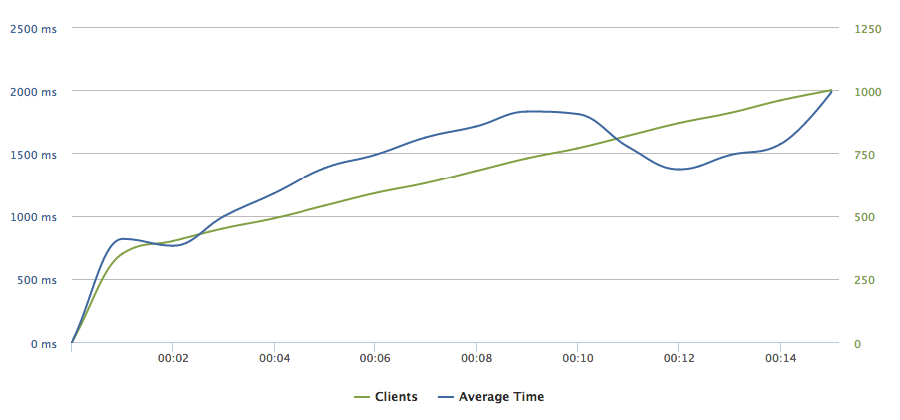
\includegraphics[scale=0.5]{figures/Nginx_FastCGI_caching.png}
\caption{Nginx with FastCGI caching: clients versus average response time}
\label{fig:nginx_fastcgi_caching}
\end{center}
\end{figure}

\begin{figure}[H]
\begin{center}
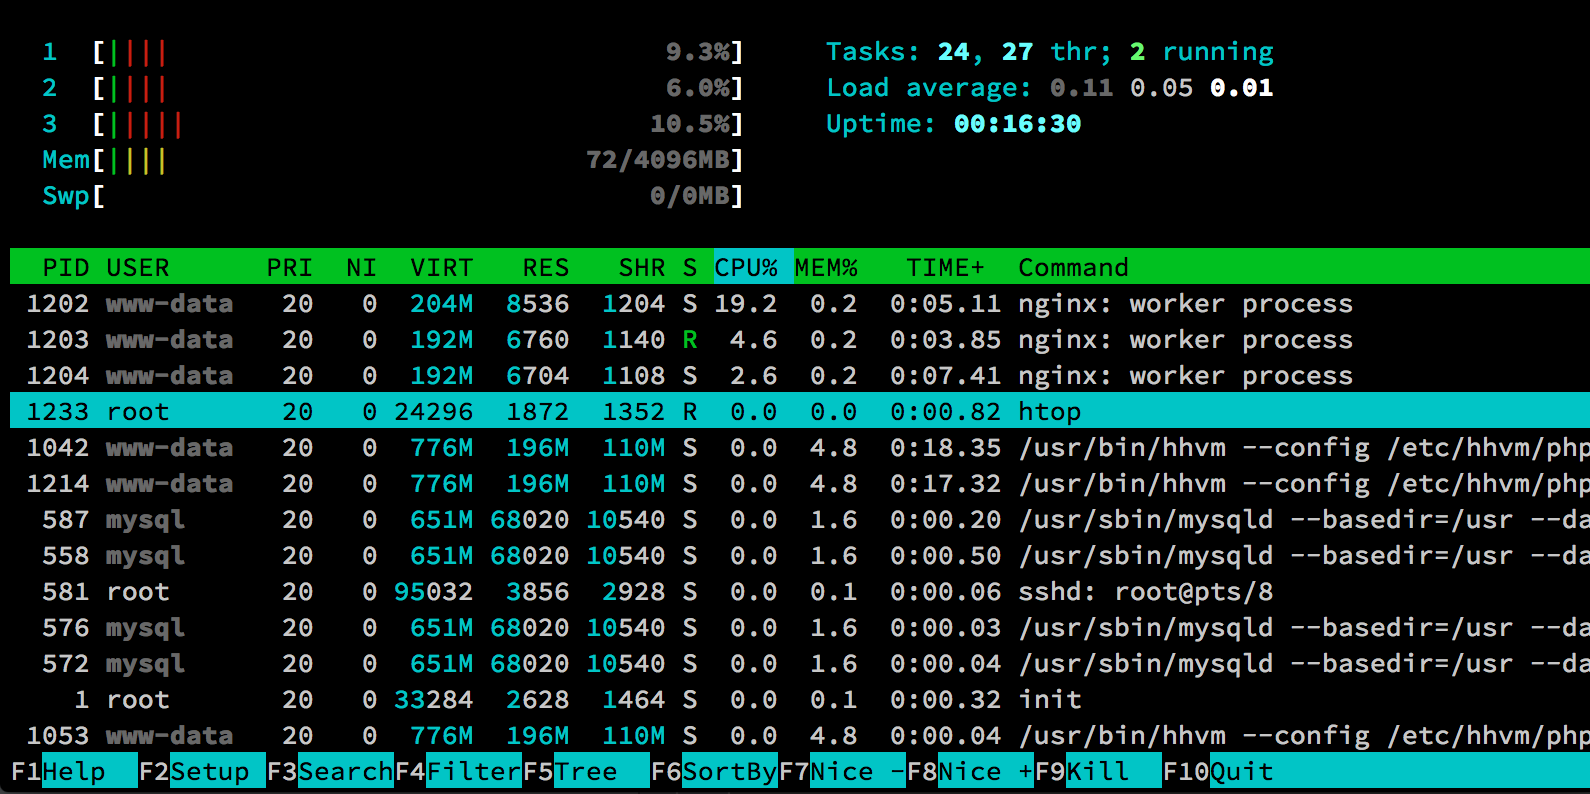
\includegraphics[scale=0.5]{figures/Nginx_FastCGI_caching_9s.png}
\caption{Nginx with FastCGI caching: Htop process viewer 9 seconds into test}
\label{fig:nginx_fastcgi_caching}
\end{center}
\end{figure}

\section{Browser caching}

Browser caching is the process of storing data in the client's browser memory. If we store the resources (CSS, JS, images and fonts) and HTML pages in the client's browser cache, the browser doesn't have to load the resources from our servers, therefore saving time and bandwidth and server processing power.

The main disadvantage of browser caching is that if addition to the resources were added or content changed, we need to revalidate the cache somehow. As the cached resources are not loaded from our server, we need to do it some other way. The preferred way to purge browser cache is to rename the resources so the browser will see them as new files which it has to load again.

To set caching, we need to specify caching options and expiration date as headers when serving files from Nginx. 

Ansible playbook..
